\chapter{Sistemas Sensoriais}\label{ch:b3:sensory-systems}

Numa noite escura um olho humano detecta um lampejo de uns poucos
fótons --- a menor quantidade de luz que a física permite detectar. O
ouvido escuta um som que move o tímpano menos que o diâmetro de um
átomo de hidrogênio e distingue um tom de outro que difere em um quinto
de por cento. Um cão segue uma trilha de algumas moléculas por
centímetro cúbico; um tubarão encontra um linguado sob a areia pelo
campo elétrico de seu batimento cardíaco. Todo sentido começa com uma
célula que converte um tipo de energia numa mudança de potencial de
membrana, e todo sentido termina como disparos num nervo; entre os dois
estão os problemas de que trata este capítulo: como um receptor
amplifica uma única molécula ou um único fóton num sinal que um
neurônio consegue ler, como uma faixa de um trilhão de vezes em
intensidade é comprimida numa taxa de algumas centenas de disparos por
segundo, como uma onda mecânica é separada por frequência, como dez mil
cheiros são distinguidos com quatrocentos receptores, e como o encéfalo,
que nunca recebe nada além de disparos, sabe de que sentido eles vieram.

\section{Princípios comuns a todos os sentidos}

\begin{definition}[Transdução, codificação e adaptação]\label{def:b3:sensory-systems:principles}
\index{transdução sensorial}\index{potencial receptor}\index{linha rotulada}\index{campo receptivo}\index{adaptação!sensorial}\index{inibição lateral}
Uma \emph{célula receptora sensorial} contém um mecanismo de
\emph{transdução} --- uma proteína ou uma cascata --- que converte um
estímulo (um fóton, uma molécula, um deslocamento, calor, um campo
elétrico) numa mudança de condutância da membrana e, portanto, num
\emph{potencial receptor}, graduado com o estímulo; a célula, ou o
neurônio sobre o qual ela faz sinapse, transforma isso num trem de
potenciais de ação cuja taxa codifica a intensidade. A
\emph{modalidade} de um sinal é dada não pelos disparos, que são
idênticos em todo nervo, mas pelo fio por onde viajam e pelo lugar do
encéfalo onde ele termina: uma \emph{linha rotulada}. Um neurônio
sensorial responde a estímulos dentro de um \emph{campo receptivo} ---
um retalho de pele, uma região do campo visual, uma faixa de
frequências --- e campos vizinhos se afinam mutuamente por
\emph{inibição lateral}, cada neurônio suprimindo os vizinhos, de modo
que bordas e contrastes ficam exagerados. A maioria dos receptores
\emph{adapta}: sua resposta a um estímulo mantido declina, de modo que
eles relatam mudança e não nível, e sua faixa de trabalho se desloca
para ficar em torno do fundo predominante.
\end{definition}

\begin{theorem}[Weber, Fechner e Stevens]\label{thm:b3:sensory-systems:weber}
\index{lei de Weber}\index{lei de Fechner}\index{lei de potência de Stevens}
A observação de Weber (1834) é que a menor mudança detectável $\Delta I$
num estímulo de intensidade $I$ é uma fração fixa dele: $\Delta I/I = k$,
com $k$ de cerca de $0.02$ para o peso, $0.08$ para o brilho, $0.1$ para
a intensidade sonora. Se cada diferença apenas perceptível for contada
como uma unidade de sensação $S$, então $\mathrm{d}S = \mathrm{d}I/
(kI)$ e
\[
S = \frac{1}{k}\ln\frac{I}{I_{0}} ,
\]
onde $I_{0}$ é o limiar: a sensação cresce com o logaritmo do estímulo
(Fechner, 1860), razão pela qual as intensidades são medidas em
decibéis e magnitudes, e pela qual uma vela acrescentada a uma vela é
notada e uma vela acrescentada a um refletor não é. Experimentos de
escalonamento direto, em que os sujeitos atribuem números às sensações,
dão, em vez disso, uma lei de potência $S \propto I^{n}$ (Stevens,
1957), com $n \approx
0.3$ para intensidade sonora e brilho, $1$ para
comprimento de linha e $3.5$ para choque elétrico; um logaritmo e uma
potência pequena são quase indistinguíveis ao longo de algumas décadas,
e as duas leis concordam no essencial: o sistema nervoso comprime.
\end{theorem}
\begin{proof}
De $\Delta I = kI$ para uma unidade de $S$, o incremento de sensação por
incremento de estímulo é $\mathrm{d}S/\mathrm{d}I = 1/(kI)$; integrando
a partir do limiar $I_{0}$, onde $S = 0$, obtém-se $S = (1/k)
\ln(I/I_{0})$. A lei de potência é a hipótese alternativa de que uma
\emph{razão} fixa de estímulos produz uma \emph{razão} fixa de
sensações, $\mathrm{d}S/S = n\,\mathrm{d}I/I$, cuja integral é $S \propto I^{n}$; para $n \to 0$, com escalonamento adequado, ela tende ao
logaritmo.
\end{proof}

\begin{omfigure}
\begin{tikzpicture}
\begin{axis}[
  width=0.68\linewidth, height=5.6cm,
  xmode=log,
  xmin=1, xmax=1e6, ymin=0, ymax=15,
  xlabel={intensidade do estímulo $I/I_{0}$}, ylabel={sensação $S$ (arbitrária)},
  xlabel style={font=\small, at={(axis description cs:0.5,-0.12)}, anchor=north}, ylabel style={font=\small},
  tick label style={font=\small}, ytick={0,5,10,15},
  clip=false,
]
\addplot[very thick, omDef, domain=1:1e6, samples=100] {ln(x)};
\addplot[very thick, omThm, domain=1:1e6, samples=100] {0.235*x^0.3 - 0.235};
\addplot[very thick, omMeth!70!black, domain=1:1e6, samples=100] {0.5*x^0.24 - 0.5};
\node[font=\scriptsize, omDef, anchor=north west] at (axis cs:2,10.2) {Fechner: $S = \ln(I/I_{0})$};
\node[font=\scriptsize, omThm, anchor=south east] at (axis cs:9e5,0.4) {Stevens: $S \propto I^{0.3}$};
\node[font=\scriptsize, omMeth!70!black, anchor=north west] at (axis cs:2,12.5) {Stevens: $S \propto I^{0.24}$};
\end{axis}
\end{tikzpicture}

{\small Compressão de uma faixa de intensidade de um milhão de vezes
numa sensação que cresce devagar: o logaritmo de Fechner e as \omterm{thm:b3:sensory-systems:weber}{leis de
potência de Stevens} com expoentes pequenos são difíceis de distinguir
ao longo de algumas décadas, e ambos dizem que os sentidos relatam
razões, e não diferenças.}
\end{omfigure}

\section{Visão}

\begin{definition}[A retina]\label{def:b3:sensory-systems:retina}
\index{retina}\index{bastonete}\index{cone}\index{fototransdução}\index{rodopsina}\index{célula ganglionar}\index{centro--periferia}
A \emph{retina} é uma lâmina de encéfalo no fundo do olho, três camadas
de células com os fotorreceptores, paradoxalmente, atrás, contra o
epitélio pigmentar. Os \emph{bastonetes} --- $10^{8}$ por olho, um
pigmento, a \emph{rodopsina} --- servem à luz fraca e saturam à luz do
dia; os \emph{cones} --- $6\times 10^{6}$, três pigmentos com picos no
azul, no verde e no vermelho, apinhados na fóvea --- servem à luz do
dia, à cor e à acuidade. A \emph{fototransdução} é uma cascata: um fóton
isomeriza o cromóforo retinal de uma rodopsina; a rodopsina ativada liga
centenas de moléculas da proteína~G transducina, cada uma das quais
ativa uma fosfodiesterase que destrói o GMP cíclico; a queda do cGMP
fecha os canais de cátions que o cGMP mantinha abertos no escuro, a
``corrente de escuro'' que entrava cessa, e a célula
\emph{hiperpolariza} --- a luz desliga um fotorreceptor, que então
libera menos glutamato. No escuro a célula está despolarizada e
liberando continuamente. O sinal passa às \emph{células bipolares} (dos
tipos ON e OFF, que o invertem ou o preservam) e daí às \emph{células
ganglionares}, um milhão por olho, cujos axônios formam o nervo óptico
--- uma compressão de cem vezes. As células horizontais e amácrinas
conectam lateralmente, e sua inibição dá a cada célula ganglionar um
\omterm{def:b3:sensory-systems:principles}{campo receptivo} de \emph{centro--periferia}: excitado por luz num disco
central e inibido por luz no anel em volta dele (ou o contrário), de
modo que a retina relata contraste local e bordas, e não luz absoluta.
\end{definition}

\begin{omfigure}
\begin{tikzpicture}[every node/.style={font=\scriptsize}, >=stealth]
  % cascade boxes with amplification numbers
  \node[draw, thick, rounded corners, fill=omProp!30, align=center] (ph) at (0,0) {1 fóton};
  \node[draw, thick, rounded corners, fill=omDef!20, align=center] (rh) at (2.6,0) {1 rodopsina*\\(metarrodopsina II)};
  \node[draw, thick, rounded corners, fill=omDef!20, align=center] (tr) at (5.6,0) {$\sim 500$ transducinas\\ativadas};
  \node[draw, thick, rounded corners, fill=omDef!20, align=center] (pde) at (8.6,0) {$\sim 500$ PDE ativas:\\$\sim 10^{5}$ cGMP hidrolisados};
  \node[draw, thick, rounded corners, fill=omThm!20, align=center] (ch) at (5.6,-2.0) {$\sim 200$ canais de cátions fecham;\\a corrente de escuro cai \qty{1}{pA}};
  \node[draw, thick, rounded corners, fill=omMeth!25, align=center] (out) at (1.4,-2.0) {hiperpolarização de \qty{1}{mV};\\menos glutamato liberado};
  \draw[->, thick] (ph) -- (rh); \draw[->, thick] (rh) -- (tr); \draw[->, thick] (tr) -- (pde);
  \draw[->, thick] (pde.south) |- (ch.east); \draw[->, thick] (ch) -- (out);
  \node[below, font=\tiny, align=center] at (7.1,-2.8) {cada etapa multiplica; toda a cascata é desligada em \qty{200}{ms} pela\\rodopsina quinase, pela arrestina e pela GTPase da transducina, e então reiniciada};
\end{tikzpicture}

{\small A \omterm{def:b3:sensory-systems:retina}{fototransdução} como amplificador. Um fóton absorvido fecha
centenas de canais através de duas etapas catalíticas, um ganho de
cerca de um milhão em moléculas --- o bastante para que um único fóton
produza uma corrente mensurável num \omterm{def:b3:sensory-systems:retina}{bastonete}.}
\end{omfigure}

\begin{theorem}[Contar fótons: a frequência de visão]\label{thm:b3:sensory-systems:hecht}
\index{detecção de fóton único}\index{curva de frequência de visão}\index{Poisson!contagem de fótons}
Um lampejo que entrega em média $a$ fótons absorvidos a um retalho de
\omterm{def:b3:sensory-systems:retina}{bastonetes} entrega, em qualquer apresentação isolada, um número $k$ que
segue uma distribuição de Poisson: $P(k) = e^{-a}a^{k}/k!$. Se o
observador relata ver o lampejo sempre que ao menos $n$ fótons são
absorvidos, a probabilidade de ver é
\[
P_{\text{ver}}(a) = 1 - \sum_{k=0}^{n-1} e^{-a}\,\frac{a^{k}}{k!} ,
\]
uma curva que sobe de $0$ a $1$ conforme $a$ aumenta e cuja
\emph{inclinação} numa escala logarítmica de $a$ depende apenas de $n$:
quanto maior a contagem-limiar, mais íngreme a curva. Ajustar a \omterm{thm:b3:sensory-systems:hecht}{curva
de frequência de visão} medida dá, portanto, $n$ sem que se saiba
quantos dos fótons entregues foram de fato absorvidos.
\end{theorem}
\begin{proof}
Os fótons de uma fonte fraca e estável chegam independentemente e ao
acaso, e o número absorvido num lampejo curto a partir de uma média $a$
é de Poisson (o limite de uma binomial com muitos fótons, cada um
absorvido com probabilidade pequena). Ver exige $k \ge n$, cuja
probabilidade é um menos a soma dos primeiros $n$ termos de Poisson.
Escalar a fonte por um fator $c$ multiplica $a$ por $c$ e desloca a
curva ao longo do eixo $\log a$ sem mudar sua forma, de modo que a forma
identifica $n$: para $n =
1$, $P = 1 - e^{-a}$ sobe ao longo de duas
décadas de $a$; para $n = 6$, sobe ao longo de menos de uma.
\end{proof}

\begin{proof}[Evidência]
Hecht, Shlaer e Pirenne (1942) sentaram observadores no escuro por meia
hora e então lançaram um minúsculo ponto verde sobre a periferia da
\omterm{def:b3:sensory-systems:retina}{retina}, rica em \omterm{def:b3:sensory-systems:retina}{bastonetes}, por um milissegundo, centenas de vezes em
várias intensidades, e registraram a fração de lampejos vistos. O
lampejo-limiar continha, na córnea, uns $90$ fótons, dos quais (após a
reflexão, a absorção nos meios do olho e a chance de $20\,\%$ de um
fóton que chega a um \omterm{def:b3:sensory-systems:retina}{bastonete} ser absorvido pela \omterm{def:b3:sensory-systems:retina}{rodopsina}) cerca de
$5$--$14$ eram absorvidos. As \omterm{thm:b3:sensory-systems:hecht}{curvas de frequência de visão} tinham a
inclinação de $n = 5$ a $7$: o observador dizia ``sim'' quando cerca de
seis \omterm{def:b3:sensory-systems:retina}{bastonetes}, dos quinhentos sob o ponto, tinham captado cada um um
único fóton. Um \omterm{def:b3:sensory-systems:retina}{bastonete} detecta um fóton; o encéfalo exige alguns em
coincidência, para manter os alarmes falsos das isomerizações
espontâneas dos \omterm{def:b3:sensory-systems:retina}{bastonetes} --- uma por \omterm{def:b3:sensory-systems:retina}{bastonete} a cada quarenta
segundos --- abaixo da taxa das estrelas.
\end{proof}

\begin{omfigure}
\begin{tikzpicture}
\begin{axis}[
  width=0.68\linewidth, height=5.6cm,
  xmode=log,
  xmin=0.1, xmax=100, ymin=0, ymax=1.05,
  xlabel={fótons absorvidos em média por lampejo, $a$}, ylabel={probabilidade de ver},
  xlabel style={font=\small, at={(axis description cs:0.5,-0.12)}, anchor=north}, ylabel style={font=\small},
  tick label style={font=\small}, ytick={0,0.5,1},
  clip=false,
]
\addplot[very thick, omDef, domain=0.1:100, samples=120] {1-exp(-x)};
\addplot[very thick, omProp, domain=0.1:100, samples=120] {1-exp(-x)*(1+x+x^2/2)};
\addplot[very thick, omThm, domain=0.1:100, samples=120] {1-exp(-x)*(1+x+x^2/2+x^3/6+x^4/24+x^5/120)};
\node[font=\scriptsize, omDef, anchor=north west] at (axis cs:0.12,0.95) {$n = 1$};
\node[font=\scriptsize, omProp, anchor=north west] at (axis cs:1.1,0.5) {$n = 3$};
\node[font=\scriptsize, omThm, anchor=north west] at (axis cs:5.5,0.45) {$n = 6$};
\end{axis}
\end{tikzpicture}

{\small \omterm{thm:b3:sensory-systems:hecht}{Curvas de frequência de visão} para limiares de um, três e seis
fótons absorvidos. Quanto mais íngreme a curva, mais fótons precisam
coincidir; os observadores de Hecht deram curvas como a vermelha.}
\end{omfigure}

\begin{omfigure}
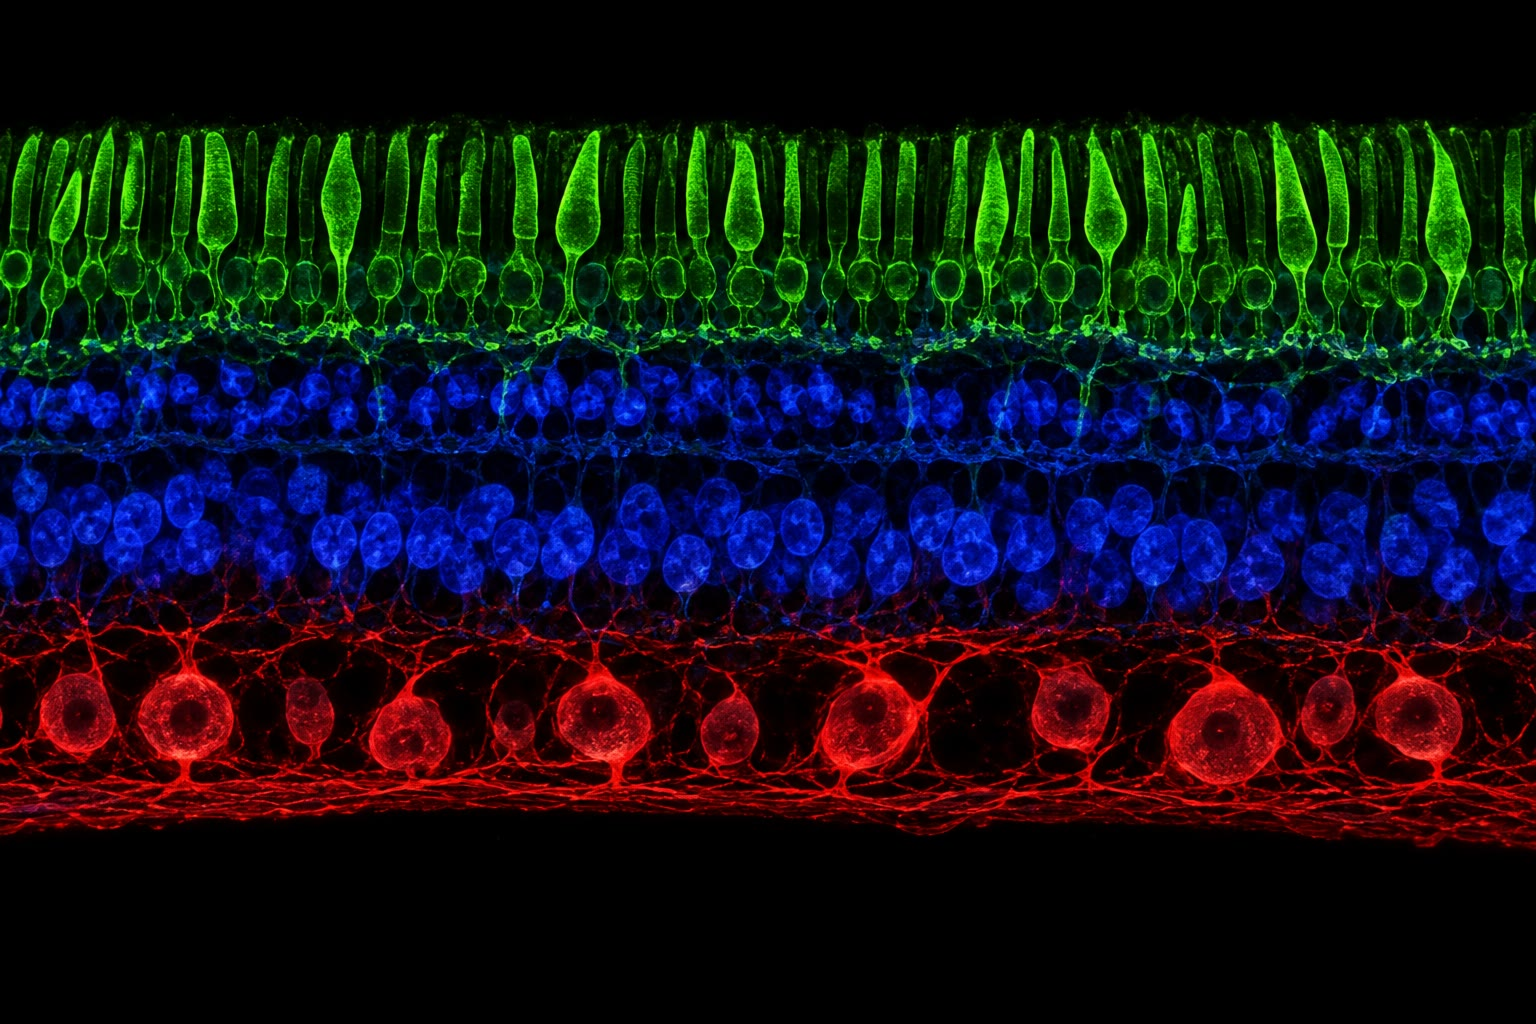
\includegraphics[width=0.46\linewidth]{images/book5/ai/b5-18-retina-section.jpg}\hspace{0.04\linewidth}
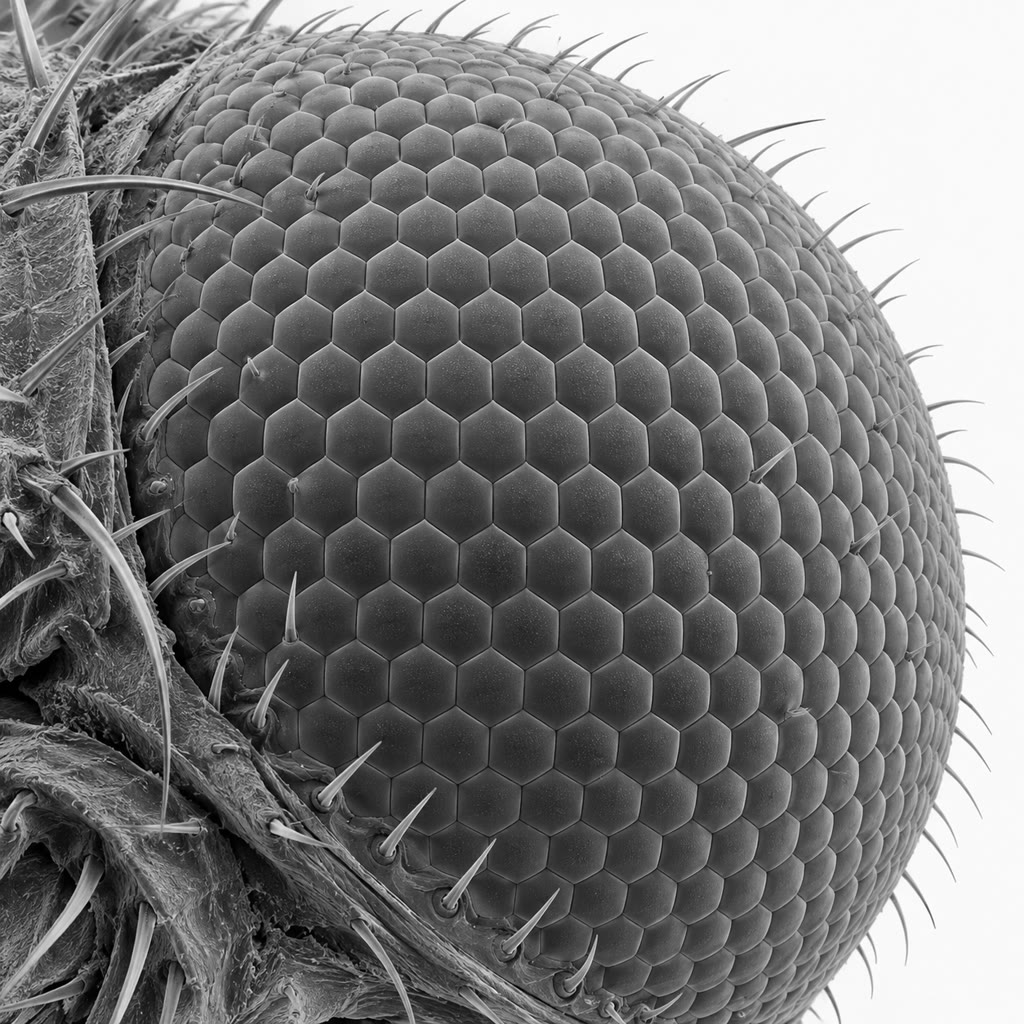
\includegraphics[width=0.36\linewidth]{images/book5/ai/b5-18-compound-eye.jpg}

{\small À esquerda: um corte da \omterm{def:b3:sensory-systems:retina}{retina}, com os fotorreceptores (verde)
ao fundo, depois as células bipolares e horizontais, depois as \omterm{def:b3:sensory-systems:retina}{células
ganglionares} (vermelho), cujos axônios partem para o encéfalo. À
direita: o olho composto de uma mosca, centenas de lentes separadas
cada uma com seus próprios receptores --- uma solução diferente para o
mesmo problema.}
\end{omfigure}

\section{Audição e equilíbrio}

\begin{definition}[A cóclea]\label{def:b3:sensory-systems:cochlea}
\index{cóclea}\index{membrana basilar}\index{tonotopia}\index{célula ciliada}\index{estereocílios}\index{ligação de ponta}\index{decibel}
O som é uma onda de pressão; o problema do ouvido é detectar variações
de pressão de algumas dezenas de micropascais no ar e separá-las por
frequência. O tímpano e os três ossículos do ouvido médio concentram a
força dos \qty{55}{mm^2} da membrana nos \qty{3}{mm^2} da janela oval,
elevando a pressão umas vinte vezes --- o casamento de impedâncias
entre o ar e o líquido do ouvido interno, sem o qual a maior parte do
som se refletiria. Dentro da \emph{cóclea}, um tubo enrolado de
\qty{35}{mm} de comprimento, a onda de pressão percorre a \emph{membrana
basilar}, que é estreita e rígida na base e larga e frouxa no ápice;
cada frequência faz a membrana vibrar mais num lugar --- as frequências
altas perto da base, as baixas perto do ápice --- um mapa
\emph{tonotópico} que o encéfalo lê como altura do som. Sobre a
membrana ficam as \emph{células ciliadas}: \num{3500} células ciliadas
internas numa única fileira, cada uma coroada por um tufo de
\emph{estereocílios} unidos ponta a ponta por finas \emph{ligações de
ponta}; curvar o tufo em direção ao seu \omterm{def:b3:cytoskeleton-motility:cilia}{cílio} mais alto estira as
ligações e abre canais de cátions em microssegundos, sem segundo
mensageiro algum, e o potássio entra vindo da endolinfa, cuja
composição incomum e cujo potencial de $+\qty{80}{mV}$ dão uma força
motriz de \qty{150}{mV}. As células ciliadas internas sinalizam ao
nervo auditivo; as \num{12000} células ciliadas externas, movidas pelo
mesmo movimento, se contraem e se alongam com o som por meio da
proteína motora prestina e bombeiam energia de volta à vibração da
membrana --- um amplificador que afina a sintonia cem vezes e é o que
falha na maioria das surdezes. A intensidade é medida em
\emph{decibéis}: $L = 10\log_{10}
(I/I_{0})$, com $I_{0} = \qty{1e-12}{W/m^2}$ o limiar da audição; o ouvido funciona ao longo de
\qty{120}{dB}, um trilhão de vezes em intensidade.
\end{definition}

\begin{omfigure}
\begin{tikzpicture}[every node/.style={font=\scriptsize}, >=stealth]
  % unrolled cochlea
  \begin{scope}
    \draw[thick, omDef, fill=omDef!10] (0,0.9) -- (7,1.4) -- (7,-1.4) -- (0,-0.9) -- cycle;
    \draw[very thick, omProp] (0,0.15) -- (7,-0.15); \draw[very thick, omProp] (0,-0.15) -- (7,0.15);
    \node[above] at (0.8,1.05) {base: estreita, rígida}; \node[above] at (6.2,1.5) {ápice: largo, frouxo};
    \node[left, align=right] at (-0.1,0) {janela oval\\(do estribo)};
    \foreach \x/\f in {0.9/\qty{16}{kHz}, 2.3/\qty{4}{kHz}, 3.8/\qty{1}{kHz}, 5.4/\qty{250}{Hz}, 6.6/\qty{60}{Hz}} { \draw[omThm, thick] (\x,-0.55) -- (\x,0.55); \node[below, omThm] at (\x,-0.65) {\f}; }
    \node[below, align=center] at (3.5,-1.7) {membrana basilar (laranja): cada frequência\\vibra mais num lugar --- a tonotopia};
  \end{scope}
  % hair cell mechanism
  \begin{scope}[xshift=8.2cm, yshift=-0.6cm]
    \draw[thick, fill=omMeth!20] (0,0) rectangle (1.6,1.2); \node[below] at (0.8,-0.05) {célula ciliada};
    \foreach \x/\h in {0.35/0.6, 0.65/0.85, 0.95/1.1, 1.25/1.35} \draw[very thick, omMeth!70!black] (\x,1.2) -- (\x,1.2+\h);
    \foreach \x/\h/\xx/\hh in {0.35/0.6/0.65/0.85, 0.65/0.85/0.95/1.1, 0.95/1.1/1.25/1.35} \draw[omThm, thick] (\x,1.2+\h) -- (\xx,1.2+\hh-0.1);
    \draw[->, thick] (1.9,2.3) -- (2.4,2.3) node[right, align=left, font=\tiny] {curvar rumo ao mais alto:\\as ligações de ponta esticam,\\os canais abrem em $\unit{\micro s}$;\\o K$^{+}$ entra (força motriz\\de \qty{150}{mV})};
    \node[above, align=center] at (0.8,2.7) {estereocílios unidos\\por ligações de ponta\\(vermelho)};
  \end{scope}
\end{tikzpicture}

{\small À esquerda: a \omterm{def:b3:sensory-systems:cochlea}{cóclea} desenrolada --- a \omterm{def:b3:sensory-systems:cochlea}{membrana basilar} passa de
rígida a frouxa, e cada frequência tem seu pico em seu próprio lugar. À
direita: um tufo de \omterm{def:b3:cytoskeleton-motility:cilia}{cílios}, cujas \omterm{def:b3:sensory-systems:cochlea}{ligações de ponta} abrem mecanicamente
os canais de transdução quando o tufo é curvado.}
\end{omfigure}

\begin{proof}[Evidência]
Von Békésy (na década de 1940) abriu as \omterm{def:b3:sensory-systems:cochlea}{cócleas} de cadáveres,
polvilhou partículas de prata sobre a \omterm{def:b3:sensory-systems:cochlea}{membrana basilar} e observou sob
luz estroboscópica enquanto tons puros criavam uma onda viajante cujo
pico ficava tanto mais perto da base quanto mais agudo o tom --- o
código de lugar, pelo qual recebeu o prêmio Nobel em 1961. Hudspeth (na
década de 1980) empurrou um único tufo de \omterm{def:b3:cytoskeleton-motility:cilia}{cílios} com uma fibra de vidro
e registrou a corrente: ela fluía em \qty{10}{\micro s} após o empurrão,
rápido demais para qualquer cascata enzimática, em proporção ao quanto
o tufo se moveu em direção à sua fileira mais alta, e sumia quando as
\omterm{def:b3:sensory-systems:cochlea}{ligações de ponta} eram cortadas com um quelante de cálcio. A abertura é
mecânica --- a ligação puxa o canal e o abre ---, razão pela qual a
audição é o mais rápido dos sentidos e pela qual seu transdutor é
destruído pelos sons altos que rompem as ligações.
\end{proof}

\begin{example}[Os números do ouvido]\label{ex:b3:sensory-systems:ear-numbers}
No limiar da audição a \omterm{def:b3:sensory-systems:cochlea}{membrana basilar} se move cerca de \qty{0.1}{nm} e
a amplitude de pressão é de \qty{20}{\micro Pa}, dois bilionésimos da
atmosférica; a \qty{120}{dB} a pressão é um milhão de vezes maior e o
movimento da membrana, de dezenas de nanômetros. Um ouvido jovem escuta
de \qty{20}{Hz} a \qty{20}{kHz} e separa tons distantes \qty{0.3}{\%}
entre si, com a discriminação do código de lugar afinada pelas \omterm{def:b3:sensory-systems:cochlea}{células
ciliadas} externas. As \num{30000} fibras do nervo auditivo disparam em
compasso com a onda de pressão até cerca de \qty{4}{kHz} (travamento de
fase), carregando temporização com precisão de dezenas de
microssegundos, a partir da qual o encéfalo calcula a direção de um som
pela diferença de chegada aos dois ouvidos --- de apenas
\qty{10}{\micro s}. Os órgãos do equilíbrio usam as mesmas \omterm{def:b3:sensory-systems:cochlea}{células
ciliadas}: nos \emph{canais semicirculares} a inércia do líquido as curva
quando a cabeça gira (aceleração angular), e nos órgãos otolíticos uma
camada de cristais de carbonato de cálcio as carrega com a gravidade e a
aceleração linear.
\end{example}

\begin{omfigure}
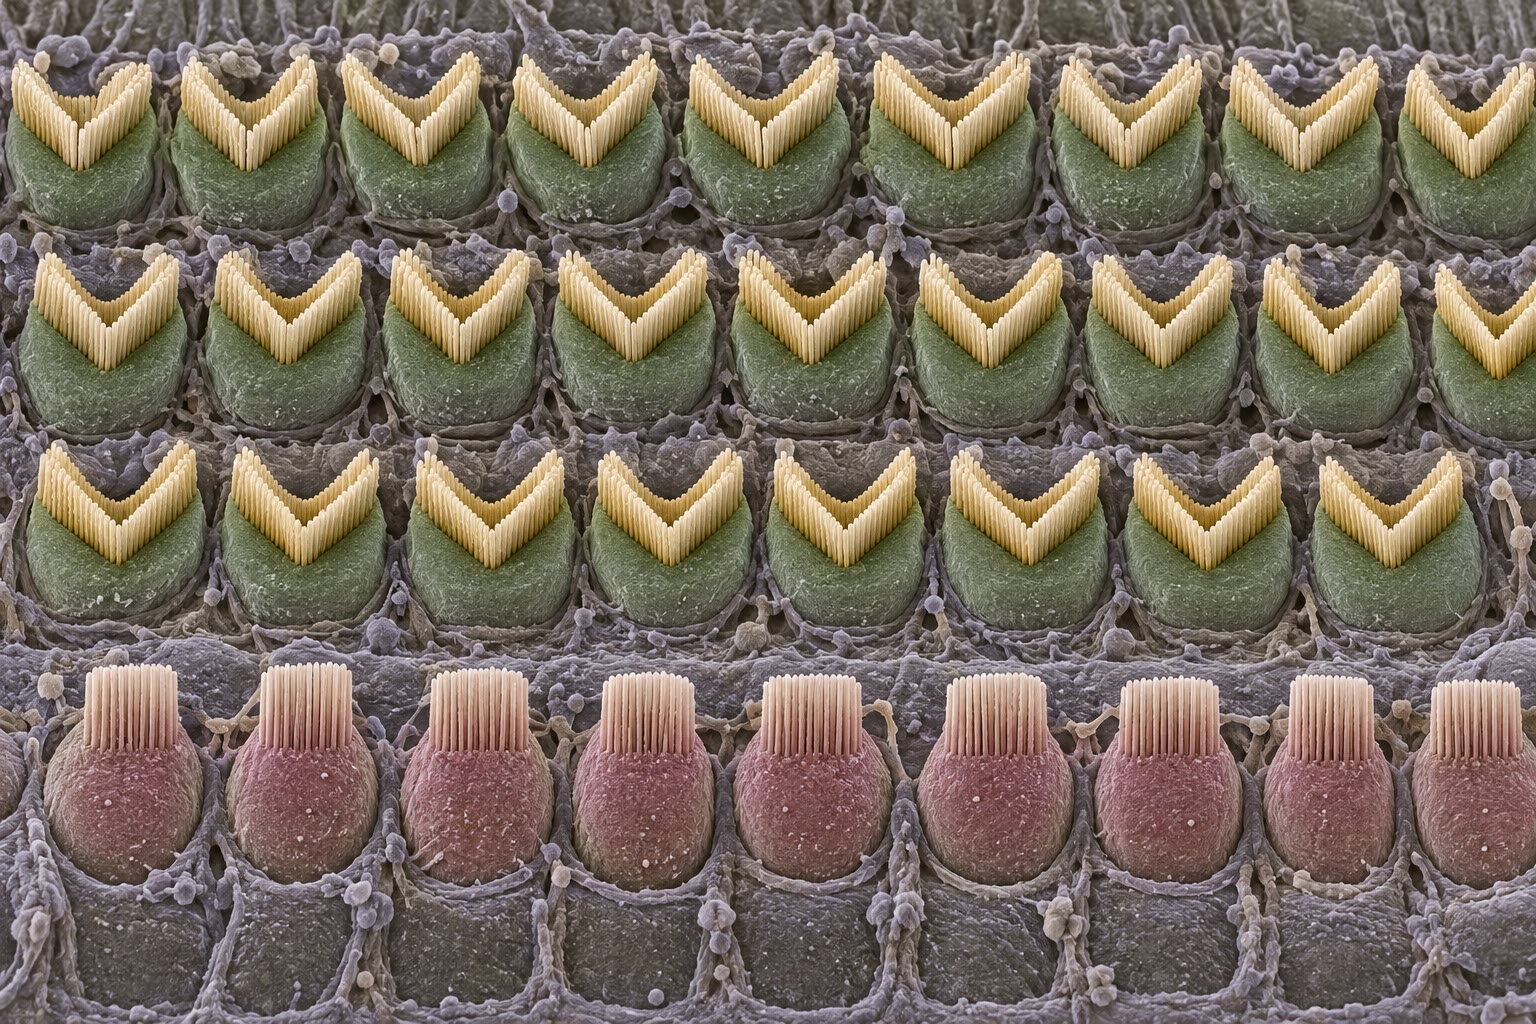
\includegraphics[width=0.54\linewidth]{images/book5/ai/b5-18-cochlea-hair-cells.jpg}

{\small O órgão de Corti visto de cima: três fileiras de \omterm{def:b3:sensory-systems:cochlea}{células
ciliadas} externas com tufos em V, uma fileira de \omterm{def:b3:sensory-systems:cochlea}{células ciliadas}
internas. As \omterm{def:b3:sensory-systems:cochlea}{ligações de ponta} de cada tufo abrem os canais; as células
externas amplificam, as internas relatam.}
\end{omfigure}

\section{Sentidos químicos}

\begin{definition}[Olfação e gustação]\label{def:b3:sensory-systems:chemical}
\index{receptor olfatório}\index{código combinatório}\index{glomérulo}\index{gustação}
O olfato começa num retalho de epitélio no alto do nariz, onde uns dez
milhões de \emph{neurônios sensoriais olfatórios} expressam, cada um, um
gene de \emph{receptor olfatório} de cerca de $400$ existentes nos
humanos (\num{1100} num camundongo, a maior família gênica dos dois
genomas) --- receptores acoplados a proteína~G que ligam moléculas
odorantes num bolso e, através do AMP cíclico, abrem um canal. Cada
receptor liga vários odorantes e cada odorante liga vários receptores,
de modo que um odor é um \emph{código combinatório}, um padrão de
atividade ao longo dos $400$ tipos de receptor, e mudar um carbono numa
molécula muda o padrão e o cheiro. Todos os neurônios que expressam um
mesmo receptor enviam seus axônios ao mesmo \emph{glomérulo} (ou aos
mesmos dois) do bulbo olfatório, de modo que o bulbo abriga um mapa em
que cada odor é um padrão espacial de glomérulos ativos, lido pelo
córtex sem passar pelo \omterm{def:b3:nervous-systems:plan}{tálamo}. A gustação é mais simples: cinco
modalidades, cada uma uma \omterm{def:b3:sensory-systems:principles}{linha rotulada} a partir de suas próprias
células receptoras --- doce, umami e amargo por receptores acoplados a
proteína~G (um receptor de doce, um de umami, uns vinte e cinco de
amargo), salgado por um canal de sódio, ácido por um canal de prótons
--- e o resto do que chamamos de sabor é olfato, chegando ao nariz pelo
fundo da boca.
\end{definition}

\begin{proof}[Evidência]
Buck e Axel (1991) raciocinaram que os receptores de odorantes seriam
receptores acoplados a proteína~G expressos apenas no epitélio
olfatório, e encontraram, por PCR com \omterm{def:b3:genetic-engineering:pcr}{iniciadores} degenerados, uma
família de centenas de genes desses, expressos ali e em nenhum outro
lugar --- os receptores do olfato, desconhecidos havia um século. A
hibridização in situ mostrou um receptor por neurônio e a \omterm{def:b3:nervous-systems:circuits}{convergência}
dos neurônios semelhantes sobre \omterm{def:b3:sensory-systems:chemical}{glomérulos} únicos; Malnic, Buck e
colaboradores (1999) registraram neurônios isolados e mostraram que cada
odorante ativava vários tipos de receptor e cada receptor, vários
odorantes --- o \omterm{def:b3:sensory-systems:chemical}{código combinatório}. Bushdid e colaboradores (2014)
pediram a sujeitos que discriminassem misturas e estimaram que os
humanos distinguem mais de um trilhão de odores, muito além dos poucos
milhares da crença comum.
\end{proof}

\begin{proposition}[A capacidade de um código combinatório]\label{prop:b3:sensory-systems:combinatorial}
\index{código combinatório!capacidade}
Com $R$ tipos de receptor, cada um ativo ou silencioso, um odor pode ser
representado por qualquer um de $2^{R}$ padrões; com $R = 400$ isso é
$10^{120}$ e, mesmo considerando apenas os padrões com exatamente $10$
tipos ativos, há $\binom{400}{10} \approx 3\times 10^{20}$. A
discriminação é limitada não pelo código, mas pelo ruído dos receptores
e pela leitura do encéfalo: um código de \omterm{def:b3:sensory-systems:principles}{linha rotulada} com um receptor
por odor permitiria $400$ cheiros; um \omterm{def:b3:sensory-systems:chemical}{código combinatório} permite mais
do que há moléculas a cheirar. O custo é que um receptor isolado diz
pouco ao encéfalo por si só; o padrão precisa ser lido como um todo, que
é o que o mapa glomerular e o córtex olfatório fazem.
\end{proposition}

\begin{omfigure}
\begin{tikzpicture}[every node/.style={font=\scriptsize}, >=stealth]
  % receptor rows, odorant columns
  \foreach \i/\lab in {1/receptor A, 2/receptor B, 3/receptor C, 4/receptor D, 5/receptor E} \node[left] at (-0.1,-0.7*\i) {\lab};
  \foreach \j/\lab in {1/hexanol, 2/heptanol, 3/octanol, 4/limoneno} \node[above, rotate=0] at (1.2*\j-0.6,-0.35) {\lab};
  \foreach \i/\j/\v in {1/1/100, 1/2/30, 2/1/60, 2/2/100, 2/3/50, 3/2/40, 3/3/100, 3/4/20, 4/3/70, 5/4/100, 1/4/30} \fill[omThm!\v] (1.2*\j-1.15,-0.7*\i-0.3) rectangle (1.2*\j-0.05,-0.7*\i+0.3);
  \foreach \i in {1,...,5} \foreach \j in {1,...,4} \draw[gray!50] (1.2*\j-1.15,-0.7*\i-0.3) rectangle (1.2*\j-0.05,-0.7*\i+0.3);
  \node[below, align=center] at (2.1,-4.1) {cada odorante ativa um conjunto de receptores,\\e cada receptor, um conjunto de odorantes:\\o cheiro é a coluna};
  % glomerular map
  \begin{scope}[xshift=9.2cm, yshift=-2.2cm]
    \draw[thick, omDef!60, fill=omDef!8] (0,0) ellipse (2.6 and 1.7); \node[above] at (0,1.75) {bulbo olfatório: glomérulos};
    \foreach \p in {(-1.8,0.6),(-1.0,1.0),(-0.2,0.7),(0.8,1.0),(1.7,0.5),(-1.6,-0.4),(-0.6,-0.6),(0.4,-0.3),(1.3,-0.7),(0.1,0.2)} \draw[omDef!70, fill=omDef!25] \p circle (0.25);
    \fill[omThm!80] (-1.0,1.0) circle (0.25); \fill[omThm!50] (0.4,-0.3) circle (0.25); \fill[omThm!80] (1.7,0.5) circle (0.25);
    \node[below, align=center] at (0,-1.8) {todos os neurônios de um tipo de receptor\\convergem para um glomérulo: um odor é\\um padrão espacial (vermelho) que o córtex lê};
  \end{scope}
\end{tikzpicture}

{\small O \omterm{def:b3:sensory-systems:chemical}{código combinatório} do olfato. À esquerda: uma matriz de
receptores por odorantes, em que cada odor é um padrão ao longo de uma
coluna. À direita: o padrão disposto sobre os \omterm{def:b3:sensory-systems:chemical}{glomérulos} do bulbo.}
\end{omfigure}

\begin{omfigure}
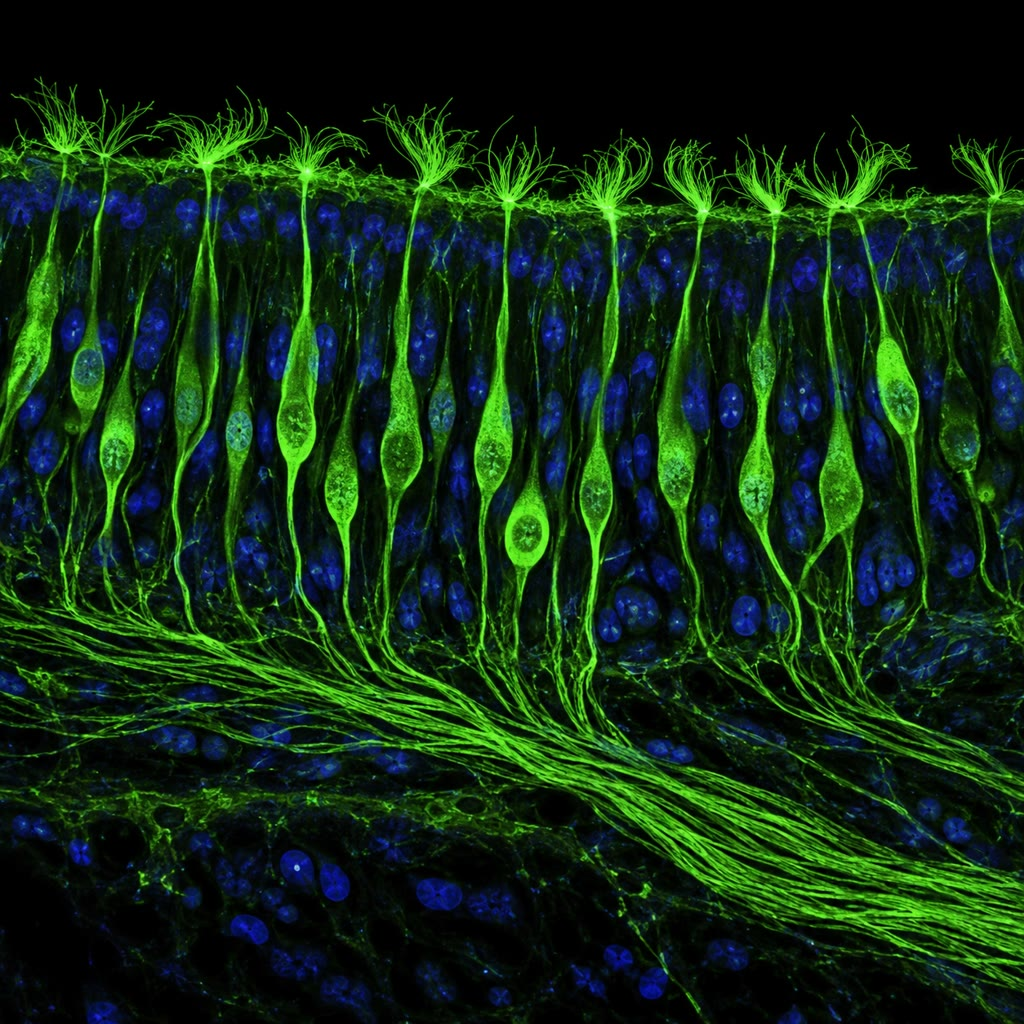
\includegraphics[width=0.40\linewidth]{images/book5/ai/b5-18-olfactory-epithelium.jpg}

{\small O epitélio olfatório: neurônios sensoriais (verde) com dendritos
ciliados na superfície, onde os odorantes se ligam, e axônios que se
agrupam abaixo rumo ao bulbo. Cada neurônio expressa um dos quatrocentos
genes de receptor.}
\end{omfigure}

\section{Tato, temperatura, dor e os sentidos que nos faltam}

\begin{definition}[Somatossensação]\label{def:b3:sensory-systems:somato}
\index{mecanorreceptor}\index{canal Piezo}\index{canal TRP}\index{nociceptor}\index{propriocepção}
A pele abriga vários tipos de \emph{mecanorreceptor}, cada um um axônio
terminando em sua própria cápsula: as células de Merkel para pressão
fina e textura (de adaptação lenta, campos pequenos), os corpúsculos de
Meissner para o toque leve e o deslizamento (de adaptação rápida), os
corpúsculos de Pacini, profundos na pele, para a vibração (de adaptação
muito rápida, campos enormes), as terminações de Ruffini para o
estiramento. O transdutor da maioria deles é o \emph{Piezo2}, um canal
iônico gigante com uma hélice de pás que abre quando a membrana é
estirada; sem ele perdem-se o tato e o sentido da posição do corpo, e o
mesmo canal, nos pulmões e na bexiga, percebe seu enchimento. A
\emph{temperatura} é percebida por canais da família TRP sintonizados em
faixas diferentes --- o TRPV1, aberto pelo calor acima de
\qty{43}{\celsius} e pela capsaicina, razão pela qual a pimenta
``queima''; o TRPM8, aberto pelo frio e pelo mentol --- e a \emph{dor},
por terminações nervosas livres, os \emph{nociceptores}, que respondem a
calor, pressão ou substâncias químicas lesivos (prótons, ATP,
bradicinina) e cujos limiares são baixados pela \omterm{def:b3:innate-immunity:inflammation}{inflamação}
(\cref{ch:b3:innate-immunity}). A \emph{propriocepção}, o sentido de
onde estão os membros, vem dos fusos musculares e dos órgãos tendinosos
do \cref{ch:b3:nervous-systems} e do Piezo2 nas cápsulas articulares. A
densidade de receptores fixa a acuidade: dois pontos a \qty{2}{mm} são
distinguidos numa ponta de dedo, e a \qty{40}{mm} nas costas.
\end{definition}

\begin{method}[Medir um sentido]\label{met:b3:sensory-systems:psychophysics}
\index{psicofísica}\index{limiar}\index{discriminação de dois pontos}
Para caracterizar um canal sensorial: (1) encontre o \emph{limiar
absoluto} apresentando estímulos de intensidade graduada muitas vezes e
ajustando a fração detectada --- a intensidade detectada metade das
vezes ---, como Hecht fez; (2) encontre o \emph{limiar diferencial} em
várias intensidades e verifique a \omterm{thm:b3:sensory-systems:weber}{lei de Weber}; (3) mapeie a
\emph{acuidade espacial} com dois estímulos a separações variáveis (o
teste de dois pontos na pele, uma grade na \omterm{def:b3:sensory-systems:retina}{retina}); (4) mapeie a
\emph{acuidade temporal} com cintilação ou cliques (uma cintilação se
funde a cerca de \qty{60}{Hz} na visão diurna); (5) num animal, registre
de fibras aferentes isoladas enquanto aplica os mesmos estímulos e
compare os limiares neurais com os comportamentais --- a psicofísica e a
fisiologia devem concordar, e onde não concordam a diferença é o que o
encéfalo acrescenta.
\end{method}

\begin{remark}[Outros animais, outros sentidos]\label{rem:b3:sensory-systems:others}
Todo sentido tratado aqui tem uma versão que algum animal levou mais
longe, e há sentidos que nos faltam. Tubarões e raias percebem os campos
de microvolts do batimento cardíaco de uma presa por canais cheios de
gelatina; os peixes elétricos leem distorções de seu próprio campo para
enxergar no escuro. As cascavéis formam imagens de presas quentes com
fossetas sensíveis ao infravermelho; morcegos e golfinhos ecolocalizam,
cronometrando ecos de seus próprios chamados com precisão de poucos
microssegundos e ajustando a frequência do chamado para rastrear uma
mariposa; as abelhas veem o ultravioleta e a polarização da luz do céu e
navegam por ela; aves e tartarugas migratórias percebem o campo
magnético da Terra por um mecanismo ainda em disputa. O nariz de um cão
tem quarenta vezes os nossos neurônios receptores e um terço de seu
encéfalo para lê-los; uma coruja ouve um rato sob a neve. Os princípios
não mudam --- um transdutor, uma \omterm{def:b3:sensory-systems:principles}{linha rotulada}, um código, compressão,
um mapa --- e a variedade é o que a evolução fez com eles.
\end{remark}

\section{Exercícios}

\begin{exercise}[$\star$]\label{exo:b3:sensory-systems:1}
Explique como o encéfalo sabe se um trem de disparos vem do olho ou do
ouvido, dado que os disparos são idênticos.
\end{exercise}

\begin{exercise}[$\star$]\label{exo:b3:sensory-systems:2}
Por que a luz hiperpolariza um fotorreceptor, e o que é a corrente de
escuro?
\end{exercise}

\begin{exercise}[$\star$]\label{exo:b3:sensory-systems:3}
Um sussurro tem \qty{20}{dB}, uma conversa \qty{60}{dB}, um show de
rock \qty{110}{dB}. Calcule a intensidade de cada um em W/m$^{2}$ e a
razão entre o mais alto e o mais baixo.
\end{exercise}

\begin{exercise}[$\star$]\label{exo:b3:sensory-systems:4}
Enuncie as cinco modalidades gustativas e seus tipos de receptor, e
explique por que um resfriado bloqueia o ``gosto'' da comida.
\end{exercise}

\begin{exercise}[$\star\star$]\label{exo:b3:sensory-systems:5}
A fração de Weber para o peso é $0.02$. Partindo de um peso de
\qty{100}{g}, quantos passos apenas perceptíveis existem entre ele e
\qty{10}{kg}? Use a fórmula de Fechner e confira contando passos de
fator $1.02$.
\end{exercise}

\begin{exercise}[$\star\star$]\label{exo:b3:sensory-systems:6}
Usando o \cref{thm:b3:sensory-systems:hecht}, calcule
$P_{\text{ver}}$ para $a = 2$, $6$ e $12$ fótons absorvidos com um
limiar de $n = 6$. Com que $a$ o lampejo é visto metade das vezes? Se
\qty{10}{\%} dos fótons na córnea são absorvidos, quantos o lampejo
precisa entregar?
\end{exercise}

\begin{exercise}[$\star\star$]\label{exo:b3:sensory-systems:7}
O ouvido médio concentra a força de \qty{55}{mm^2} em \qty{3}{mm^2} com
uma alavanca de $1.3$. Por que fator a pressão é elevada, e em
decibéis? Por que o ouvido de uma pessoa com os ossículos fundidos
(otosclerose) é dezenas de decibéis mais surdo?
\end{exercise}

\begin{exercise}[$\star\star$]\label{exo:b3:sensory-systems:8}
Explique por que a corrente de transdução de uma \omterm{def:b3:sensory-systems:cochlea}{célula ciliada} aparece
em microssegundos enquanto a de um fotorreceptor leva dezenas de
milissegundos, e o que cada sentido ganha com seu projeto.
\end{exercise}

\begin{exercise}[$\star\star$]\label{exo:b3:sensory-systems:9}
Um camundongo tem \num{1100} tipos de receptor e um humano, $400$. Se um
odor ativa cerca de \qty{5}{\%} dos tipos, quantos padrões exatamente
desse tamanho estão disponíveis para cada um (use $\binom{R}{k}$ com
$k = 0.05R$ e a aproximação de Stirling $\ln\binom{R}{k} \approx R\,H(k/R)$
com $H(p) = -p\ln p - (1-p)\ln(1-p)$)?
\end{exercise}

\begin{exercise}[$\star\star\star$]\label{exo:b3:sensory-systems:10}
Um \omterm{def:b3:sensory-systems:retina}{bastonete} isomeriza uma \omterm{def:b3:sensory-systems:retina}{rodopsina} espontaneamente uma vez a cada
\qty{40}{s} no escuro. Num retalho de $500$ \omterm{def:b3:sensory-systems:retina}{bastonetes} observado por uma
janela de \qty{0.1}{s}, qual é o número médio de eventos espontâneos, e
a probabilidade de que seis ou mais ocorram por acaso? Explique por que
o encéfalo põe o limiar em cerca de seis, e não em um.
\end{exercise}

\begin{exercise}[$\star\star\star$]\label{exo:b3:sensory-systems:11}
O nervo auditivo trava seus disparos na fase do som até \qty{4}{kHz},
com um jitter de cerca de \qty{20}{\micro s}. O som viaja a
\qty{340}{m/s} e os ouvidos estão a \qty{20}{cm} um do outro. Qual é o
maior atraso interaural, que resolução angular uma discriminação de
\qty{10}{\micro s} dá perto da linha média, e por que é o código de
lugar, e não a temporização, que serve acima de \qty{4}{kHz}?
\end{exercise}

\begin{exercise}[$\star\star\star$]\label{exo:b3:sensory-systems:12}
A \omterm{def:b3:sensory-systems:principles}{inibição lateral} faz um campo cinza uniforme ao lado de um escuro
parecer mais claro na borda. Modele uma fileira de receptores, cada um
excitado por sua própria luz $I_{i}$ e inibido por uma fração $w$ da de
cada vizinho, $r_{i} = I_{i} - w(I_{i-1} + I_{i+1})$, e calcule a
resposta ao longo de um degrau de $I = 1$ a $I = 2$ com $w = 0.2$. O que
a \omterm{def:b3:sensory-systems:retina}{retina} ganha e o que perde com isso?
\end{exercise}

\section{Problema: Uma Vela Vista de Longe}

\begin{problem}[{Problema de fim de semana --- os fótons de uma vela
contados até um olho distante, a detecção do lampejo calculada pela
estatística de Poisson e pelo amplificador do bastonete, os decibéis de
um show convertidos em movimento do tímpano e corrente de célula
ciliada, e o código de um nariz enumerado, terminando na distância em
que a vela é vista, na pressão no tímpano e nos padrões que um nariz
consegue formar}]
\label{pb:b3:sensory-systems:1}
Dados: uma vela emite cerca de \qty{0.01}{W} de luz visível, a
\qty{550}{nm} (energia do fóton $3.6\times 10^{-19}$ J). Uma pupila
adaptada ao escuro tem \qty{7}{mm} de diâmetro; \qty{10}{\%} dos fótons
que entram no olho são absorvidos pela \omterm{def:b3:sensory-systems:retina}{rodopsina}; o olho integra ao
longo de \qty{0.1}{s}; o limiar é de $6$ fótons absorvidos. Cada fóton
absorvido fecha $200$ canais e reduz a corrente de escuro em
\qty{1}{pA} por \qty{0.2}{s}; a corrente de escuro de um \omterm{def:b3:sensory-systems:retina}{bastonete} é de
\qty{30}{pA}. Som: $I_{0} =
\qty{1e-12}{W/m^2}$; o tímpano tem área de
\qty{55}{mm^2}; um tufo de \omterm{def:b3:cytoskeleton-motility:cilia}{cílios} de \qty{5}{\micro m} de altura se
deflete \qty{0.3}{nm} no limiar. Olfação: $R = 400$ receptores; a
corrente de transdução de uma \omterm{def:b3:sensory-systems:cochlea}{célula ciliada} é de \qty{100}{pA} na
saturação.

\medskip
\noindent\textbf{Parte I --- Fótons.}
\begin{enumerate}
  \item Quantos fótons por segundo a vela emite?
  \item À distância $d$ os fótons se espalham por uma esfera de área
        $4\pi d^{2}$. Quantos entram na pupila por segundo a
        \qty{1}{km}? E a \qty{10}{km}?
  \item Quantos são absorvidos numa janela de integração em cada
        distância? A vela é vista (limiar $6$)?
  \item Encontre a distância em que o número médio absorvido numa janela
        é igual a $6$. Com a estatística de Poisson, que fração das
        janelas ultrapassa o limiar ali?
  \item À distância da questão 4, qual é a probabilidade de que uma dada
        janela de \qty{0.1}{s} não contenha fóton algum? Por que uma
        estrela fraca parece cintilar?
  \item Sob lua cheia os mesmos \omterm{def:b3:sensory-systems:retina}{bastonetes} absorvem $10^{4}$ fótons do
        céu por janela. Explique por que a vela a \qty{10}{km} fica
        então invisível, embora entregue os mesmos fótons.
\end{enumerate}

\medskip
\noindent\textbf{Parte II --- O amplificador do \omterm{def:b3:sensory-systems:retina}{bastonete}.}
\begin{enumerate}[resume]
  \item Um fóton fecha $200$ canais e reduz a corrente em \qty{1}{pA}.
        Que corrente um canal conduz, e quantos cátions por segundo são
        ($e = \qty{1.6e-19}{C}$)?
  \item Que fração da corrente de escuro um fóton remove? Quantos fótons
        simultâneos desligariam o \omterm{def:b3:sensory-systems:retina}{bastonete} por completo (saturação)?
  \item A resposta dura \qty{0.2}{s}. Quantos cátions um fóton impede de
        entrar? Qual é o ganho em carga por fóton?
  \item À luz do dia $10^{5}$ fótons por segundo chegam a um \omterm{def:b3:sensory-systems:retina}{bastonete}. O
        que acontece com ele, e por que os \omterm{def:b3:sensory-systems:retina}{cones}, que adaptam e saturam
        menos, são os receptores diurnos?
  \item Os \omterm{def:b3:sensory-systems:retina}{cones} precisam de cerca de $100$ fótons para sinalizar.
        Explique, em termos do compromisso entre sensibilidade e
        rapidez, por que os \omterm{def:b3:sensory-systems:retina}{cones} respondem em \qty{20}{ms} e os
        \omterm{def:b3:sensory-systems:retina}{bastonetes} em \qty{200}{ms}.
  \item Uma \omterm{def:b3:sensory-systems:retina}{rodopsina} isomeriza espontaneamente uma vez a cada
        \qty{40}{s}. Nos $10^{8}$ \omterm{def:b3:sensory-systems:retina}{bastonetes} de um olho, quantos fótons
        falsos por segundo a \omterm{def:b3:sensory-systems:retina}{retina} gera, e por que isso não cega de
        ruído o olho no escuro? (Pense no limiar e no \omterm{def:b3:sensory-systems:principles}{campo receptivo}.)
\end{enumerate}

\medskip
\noindent\textbf{Parte III --- Decibéis.}
\begin{enumerate}[resume]
  \item Um show a \qty{110}{dB}: intensidade em W/m$^{2}$ e potência que
        incide sobre um tímpano.
  \item Quanta energia acústica o tímpano recebe num show de duas horas?
        Compare com a energia de uma gota de chuva em queda
        (\qty{1e-4}{J}).
  \item O limiar da audição a \qty{0}{dB}: potência sobre o tímpano e
        energia por \qty{10}{ms} --- compare com a energia de um fóton
        visível.
  \item O tufo de \omterm{def:b3:cytoskeleton-motility:cilia}{cílios} se deflete \qty{0.3}{nm} no limiar, sobre uma
        altura de \qty{5}{\micro m}. Que ângulo é esse, em graus?
        Compare a deflexão com o diâmetro de um átomo de hidrogênio
        (\qty{0.1}{nm}).
  \item A exposição prolongada acima de \qty{85}{dB} danifica as \omterm{def:b3:sensory-systems:cochlea}{células
        ciliadas}, e as \omterm{def:b3:sensory-systems:cochlea}{células ciliadas} não se regeneram nos mamíferos.
        Duas horas a \qty{110}{dB} entregam tanta energia quanto quantas
        horas a \qty{85}{dB}?
  \item A faixa da audição é de \qty{120}{dB}. Quantos passos apenas
        perceptíveis de intensidade sonora são esses, se a fração de
        Weber para a intensidade é de cerca de $0.25$ (um \omterm{def:b3:sensory-systems:cochlea}{decibel})?
\end{enumerate}

\medskip
\noindent\textbf{Parte IV --- O código do olfato.}
\begin{enumerate}[resume]
  \item Com $400$ receptores, cada um ligado ou desligado, quantos
        padrões? Escreva a resposta como uma potência de dez.
  \item Se um odor tipicamente ativa $20$ receptores, quantos padrões
        distintos desses existem ($\binom{400}{20}$, use Stirling ou
        logaritmos)?
  \item Dois odorantes compartilham $15$ de seus $20$ receptores.
        Proponha uma medida da distância entre eles no código e explique
        por que eles cheiram parecido.
  \item Os humanos discriminam cerca de um trilhão de odores. Que fração
        dos padrões da questão 20 é isso, e o que limita o número a
        tanto abaixo da capacidade do código?
  \item Um camundongo com \num{1100} receptores: quantos padrões de $20$
        a mais que um humano, como potência de dez?
  \item Uma mutação deleta um gene de receptor. Preveja seu efeito sobre
        a capacidade de cheirar em geral e sobre a percepção de um
        odorante que liga fortemente esse receptor (anosmia específica).
  \item Resuma: a distância em que a vela é vista (questão~4), a energia
        acústica no tímpano no limiar em \qty{10}{ms} (questão~15) e o
        número de padrões de vinte receptores que um nariz humano
        consegue formar (questão~20).
\end{enumerate}
\end{problem}
